\documentclass{article}
\usepackage{fancyhdr}
\usepackage{extramarks}
\usepackage{amsmath}
\usepackage{amsthm}
\usepackage{amsfonts}
\usepackage{tikz}
\usepackage[plain]{algorithm}
\usepackage{algpseudocode}
\usepackage{enumerate}
\usepackage{tikz}
\usepackage{xifthen}
\usepackage{xparse}
\usepackage{amsmath, amssymb}
\usepackage{lipsum}

\usetikzlibrary{automata,positioning}

%
% Basic Document Settings
%  

\topmargin=-0.45in
\evensidemargin=0in
\oddsidemargin=0in
\textwidth=6.5in
\textheight=9.0in
\headsep=0.25in

\linespread{1.1}

\pagestyle{fancy}
\lhead{\hmwkAuthorName}
\chead{\hmwkClass: \hmwkTitle}
\rhead{\firstxmark}
\lfoot{\lastxmark}
\cfoot{\thepage}

\renewcommand\headrulewidth{0.4pt}
\renewcommand\footrulewidth{0.4pt}

\setlength\parindent{0pt}

%
% Create Problem Sections
%

\newcommand{\enterProblemHeader}[1]{
    \nobreak\extramarks{}{Problem \arabic{#1} continued on next page\ldots}\nobreak{}
    \nobreak\extramarks{Problem \arabic{#1} (continued)}{Problem \arabic{#1} continued on next page\ldots}\nobreak{}
}

\newcommand{\exitProblemHeader}[1]{
    \nobreak\extramarks{Problem \arabic{#1} (continued)}{Problem \arabic{#1} continued on next page\ldots}\nobreak{}
    \stepcounter{#1}
    \nobreak\extramarks{Problem \arabic{#1}}{}\nobreak{}
}

\newcommand*\circled[1]{\tikz[baseline=(char.base)]{
		\node[shape=circle,draw,inner sep=2pt] (char) {#1};}}


\setcounter{secnumdepth}{0}
\newcounter{partCounter}
\newcounter{homeworkProblemCounter}
\setcounter{homeworkProblemCounter}{1}
\nobreak\extramarks{Problem \arabic{homeworkProblemCounter}}{}\nobreak{}

%
% Homework Problem Environment
%
% This environment takes an optional argument. When given, it will adjust the
% problem counter. This is useful for when the problems given for your
% assignment aren't sequential. See the last 3 problems of this template for an
% example.
%

\NewDocumentEnvironment{homeworkProblem}{s m}{
    \IfBooleanT{#1}{\newpage}
    \section{Problem \arabic{homeworkProblemCounter} {\small (#2)}}
    \setcounter{partCounter}{1}
    \enterProblemHeader{homeworkProblemCounter}

}{
    \exitProblemHeader{homeworkProblemCounter}
}

%
% Homework Details
%   - Title
%   - Due date
%   - Class
%   - Instructor
%   - Class number
%   - Name
%   - Student ID

\newcommand{\hmwkTitle}{Homework\ \#7}
\newcommand{\hmwkDueDate}{September 18, 2022}
\newcommand{\hmwkClass}{Probability and Mathematical Statistics}
\newcommand{\hmwkClassInstructor}{Professor Ziyu Shao}

\newcommand{\hmwkClassID}{\circled{0}}

\newcommand{\hmwkAuthorName}{Zhu Zhelin}
\newcommand{\hmwkAuthorID}{2021533077}

%
% Title Page
%

\title{
    \vspace{2in}
    \textmd{\textbf{\hmwkClass:\\  \hmwkTitle}}\\
    \normalsize\vspace{0.1in}\small{Due\ on\ \hmwkDueDate\ at 11:59am}\\
   \vspace{2in}\Huge{\hmwkClassID}\\   
   \vspace{2in}
}

\author{
	Name: \textbf{\hmwkAuthorName} \\
	Student ID: \hmwkAuthorID}
\date{}


\renewcommand{\part}[1]{\textbf{\large Part (\alph{partCounter})}\stepcounter{partCounter}\\}

%
% Various Helper Commands
%

% Useful for algorithms
\newcommand{\alg}[1]{\textsc{\bfseries \footnotesize #1}}
% For derivatives
\newcommand{\deriv}[1]{\frac{\mathrm{d}}{\mathrm{d}x} (#1)}
% For partial derivatives
\newcommand{\pderiv}[2]{\frac{\partial}{\partial #1} (#2)}
% Integral dx
\newcommand{\dx}{\mathrm{d}x}
% Alias for the Solution section header
\newcommand{\solution}{\textbf{\Large Solution}}
% Probability commands: Expectation, Variance, Covariance, Bias
\newcommand{\E}{\mathrm{E}}
\newcommand{\Var}{\mathrm{Var}}
\newcommand{\Cov}{\mathrm{Cov}}
\newcommand{\Bias}{\mathrm{Bias}}

\begin{document}

\maketitle
\pagebreak

% Problem 1
\begin{homeworkProblem}{{\color{blue}mention the source of question}, \textit{e.g.}, BH CH0 \#1}

	\begin{enumerate}[(a)]
		\item To show it \begin{enumerate}[(i)]
		\item When X and Y are both discrete by definition,$P(Y=y|X=x)=\frac{P(Y=y,X=x)}{P(X=x)}$ \\since $P(X=x|Y=y)=\frac{P(X=x,Y=y)}{P(Y=y)}$,so $P(Y=y|X=x)=\frac{P(X=x|Y=y)P(Y=y)}{P(X=x)}$
	\item When Y is continuous,X is discrete,
	\begin{equation}	
	\begin{aligned}
&f_Y(y|X=x)=\lim_{\epsilon\to 0}\frac{P(y-\epsilon\leq Y \leq y+\epsilon|X=x)}{2\epsilon}\hfill
\\ &=\lim_{\epsilon\to 0}\frac{P( y-\epsilon\leq Y\leq y+\epsilon,X=x)}{2\epsilon\cdot P(X=x)}
\\ &= \lim_{\epsilon\to 0}\frac{P(X=x|y-\epsilon\leq Y\leq y+\epsilon)\cdot P(y-\epsilon\leq Y\leq y+\epsilon )}{P(X=x)\cdot 2\epsilon}
\\ &=\frac{P(X=x|Y=y)f_Y(y)}{P(X=x)}		
\end{aligned}
\end{equation}
\item  when  X continuous ,Y discrete\begin{equation}
\begin{aligned}
&P(Y=y|X=x)=\lim_{\epsilon\to 0}P(Y=y|x-\epsilon\leq X\leq x+\epsilon)
\\ &=\lim_{\epsilon\to 0}\frac{P(Y=y,x-\epsilon\leq X\leq x+\epsilon)}{P( x-\epsilon \leq X\leq x+\epsilon )}
\\ &=\lim_{\epsilon \to 0}\frac{\frac{P(x-\epsilon\leq X\leq x+\epsilon|Y=y}{2\epsilon)}P(Y=y)}{ \frac{P(x-\epsilon\leq X\leq X+\epsilon)}{2\epsilon}}
\\  &=\frac{f_X(x|Y=y)P(Y=y)}{f_X(x)}
\end{aligned}
\end{equation}
\item when X and Y are continous ,by definition $f_{Y|X}(y|x)=\frac{f_{X,Y}(x,y)}{f_X(x)}$,since $f_{X,Y}(x,y)=f_{X|Y}(x|y)f_Y(y)$,so $f_{Y|X}(y|x)=\frac{f_{X|Y}(x|y)f_{Y}(y)}{f_{X}(x)}$
\end{enumerate}
\newpage
\item \begin{enumerate}[(i)]
\item since conditional PMF is also valid PMF  so,$\sum_{y}P(Y=y|X=x)=1=\sum_{y}\frac{P(Y=y,X=x)}{P(X=x)}=1$ thus $\sum_{y}P(Y=y,X=x)=P(X=x)$ ,then $$\sum_{y}P(X=x|Y=y)P(Y=y)=\sum_{y}P(X=x,Y=y)=P(X=x)$$
\item When X is discrete,Y is continous
\begin{equation}
	\begin{aligned}
& P(X=x|Y=y)=\frac{f_Y(y|X=x)}{f_Y(y)}\cdot P(X=x)
\\& \int_{-\infty}^{+\infty}P(X=x|Y=y)f_Y(y)dy=\int_{-\infty}^{+\infty}P(X=x)f_Y(y|X=x)dy
\\& =P(X=x)
	\end{aligned}
\end{equation}
\item when X is continous ,and Y is discrete, $f_X(x)=\lim_{\epsilon\to 0}\frac{P(x-\epsilon\leq X\leq x+\epsilon)}{2\epsilon}$\\
=$\sum_{y}\frac{P(x-\epsilon\leq X\leq x+\epsilon|Y=y)P(Y=y)}{2\epsilon}=\sum_{y} f_{X}(x|Y=y)P(Y=y)$
\item when X and Y are both continous $f_{X}(x)=\int _{-\infty}^{+\infty}f_{X,Y}(X=x,Y=y)dy$ using bayes' rule
\\=$\int _{-\infty}^{+\infty}f_{X|Y}(x|y)f_{Y}(y)dy$ 
	\end{enumerate}
\end{enumerate}
\end{homeworkProblem}

% Problem 2
\begin{homeworkProblem}*{BH CH0 \#2}
\solution\\
\begin{enumerate}[(a)]
	\item To find CDF we can integral PDF $F(x)=\int _{-\infty}^{x}\frac{1}{\pi(1+t^2)}dt
	=\frac{tan^{-1}(x)}{\pi}+\frac{1}{2}$
	\item by using integral F(x)=0(when $x<1$),F(x)=$\int_{1}^{x}at^{-a-1}dt$=$1-x^{-a}$(when x$\geq 1$) ,to check the validation,$f(x)\geq 0 for all x$,$\lim_{x\to \infty}F(x)=1-0=1$
	\item let Y=max(Z-c,0) then we know when Z$\geq c Y=Z-c$ else Y=0 then $E(Y)=\int_{c}^{\infty}(z-c)\frac{1}{\sqrt{2\pi}}e^{-\frac{z^2}{2}}dz=\frac{1}{\sqrt{2\pi}}e^{-\frac{c^2}{2}}-c(1-\Phi(c))$ 
=$\varphi(c)-c+c\Phi(c)$
\end{enumerate}



\end{homeworkProblem}


\begin{homeworkProblem}*{BH CH0 \#3}
	\begin{enumerate}[(a)]
		\item from drawing the line ,I can easily get that $(G\delta t=T$( the $G_{th}$ failure,the first trial begin at when t=0)
	\item P($T>t$)=P(G$\Delta t>t$),considering when t=k$\Delta t,k\in Z$,then $G\geq k+1$,when $(k-1)\Delta t<t<k\Delta t$,we calculate $G\geq k$,so we just choose $G\geq \lfloor \frac{t}{\Delta t}\rfloor+1$,since G satify Geometry distrbution so $P(G\geq \lfloor \frac{t}{\Delta t}\rfloor+1)$
=$\sum_{k=\lfloor \frac{t}{\Delta t}\rfloor+1}^{\infty}(1-\lambda \Delta t)^{k}\lambda \Delta t=(1-\lambda \Delta t)^{\lfloor \frac{t}{\Delta t}\rfloor+1}$	,then CDF is $1-(1-\lambda \Delta t)^{\lfloor \frac{t}{\Delta t}\rfloor+1}$
\item considering the limit of $\lim_{\Delta t\to 0}(1-\lambda \Delta t)^{ \frac{t}{\Delta t} }\leq\lim_{\Delta t\to 0}(1-\lambda \Delta t)^{\frac{t}{\Delta t} +1}=\lim((1-\lambda\Delta t)^{\frac{1}{\lambda \Delta t}})^{\lambda t}(1-\lambda\Delta t)=e^{-\lambda t}$,so the CDF is $1-e^{-\lambda t}$satisfy $Expo(\lambda)$
\end{enumerate}
\end{homeworkProblem}
\begin{homeworkProblem}*{BH CH0 \#4}
	\begin{enumerate}[(a)]
\item \begin{figure}[htbp]
	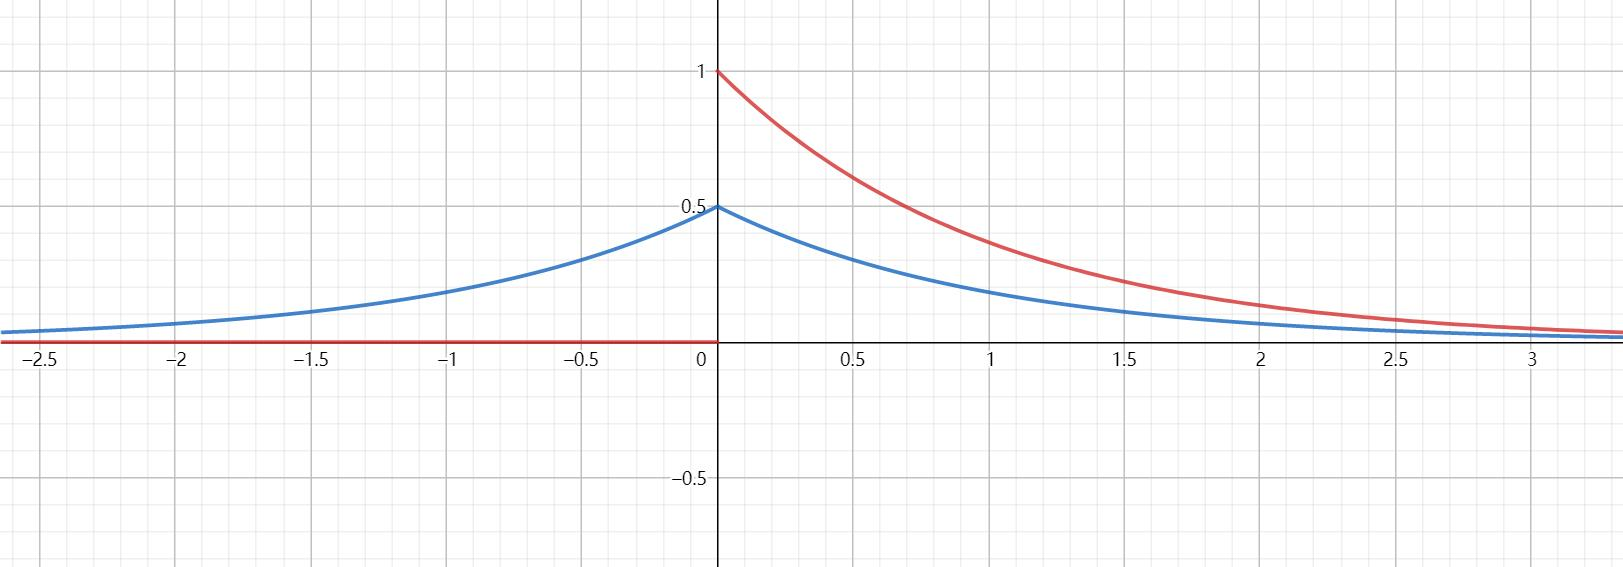
\includegraphics{p4.jpg}
\end{figure}
The amplitude is half of the expo distribution,so the right of laplace distribution is actually exponential distribution but with an area smaller.
\item using lotp P(SX$>t$)=P(X$>$t|S=1)P(S=1)+P(X$<$-t|S=-1)P(S=-1)=$\frac{1}{2}(P(X>t)+P(X<-t))$ when t$>$0,P(S$X>$t)=$\frac{e^{-t}}{2}$ when t $\leq$0 then P(SX$>$t)=$\frac{2-e^t}{2}$,so we can get the PDF equal to the laplace function
\end{enumerate}
\end{homeworkProblem}

\begin{homeworkProblem}*{BH CH0 \#5}
\begin{enumerate}[(a)]
	\item $r=\frac{1}{n}\sum(x_i-\overline{x})(y_i-\overline{y})=\frac{1}{n}\sum(x_iy_i-\overline{x}y_i-\overline{y}x_i+\overline{xy})=\frac{1}{n}\sum x_iy_i-\frac{\overline{x}\sum{y_i}}{n}-\frac{\overline{y}\sum{x_i}}{n}+\overline{x}\cdot\overline{y}=\overline{xy}-\overline{x}\cdot\overline{y}=E(XY)-E(X)E(Y)=COV(X,Y)$
	\item to consider the average signed area of expectation formed by $(X,Y),(\hat{X},\hat{Y})$ which indicates $E((X-\hat{X})(Y-\hat{Y}))$ since two trial is independent there are $\frac{1}{n^2}$possibility to choose $(x_i,y_i),(x_j,y_j)$ so the total expectation is $\frac{\sum_{j}\sum_{i}(x_i-x_j)(y_i-y_j)}{n^2}=\frac{\sum_{j}\sum_{i}x_iy_i-x_jy_i-y_ix_i+x_jy_i}{n^2}=2\overline{xy}-2\overline{x}\cdot\overline{y}=2Cov(X,Y)=2r$ ,so the sample variance is a constant time of the total signed area of the rectangle 
	\item \begin{enumerate}[(i)]
		\item since it is the constant time of the average signed area of two indepent trials,changing the x and y axis doesn't change the area,so $Cov(W1,W2)=Cov(W2,W1)$
	\item the linearscaling of the random variable will also lead to the area to be extended to $a_1a_2$ times,so $Cov(a1W1,a2W2)=a1a2Cov(W1,W2)$
	\item  the translation of axis doesn't change the area ,so $Cov (W 1 + a1 , W 2 + a2 ) = Cov (W 1 , W 2 ) $
	\item  the area with x=x1,y=y1+y2, is the same area as two area sum up x=x1,y=y1,and x=x1,y=y2,so Cov(W1,W2+W3)=Cov(W1,W2)+Cov(W1,W3)
	\end{enumerate}
\end{enumerate}
\end{homeworkProblem}
\end{document}
